\documentclass[11pt]{article}


\usepackage[utf8]{inputenc} % remove if using XeLaTeX or LuaLaTeX
\usepackage[T1]{fontenc}

% Layout & graphics
\usepackage[a4paper, total={7.5in, 9in}]{geometry}
\usepackage{graphicx}              % images
\usepackage[dvipsnames,table]{xcolor} % single xcolor invocation (keeps table option)

% Math & symbols
\usepackage{amsmath}
\usepackage{amssymb}
\usepackage{gensymb}

% Typography & layout helpers
\usepackage{microtype}
\usepackage{float}                 % [H] placement
\usepackage{caption}
\usepackage{subcaption}            % modern subfigure support (do NOT load subfig)
\usepackage{multirow}
\usepackage{titlesec}

\usepackage{lmodern}
\usepackage{microtype}

\definecolor{xppblue}{RGB}{37, 150, 190}

\begin{document}

\begin{table}[H]
\centering
\begin{tabular}{|p{4cm}|p{8cm}|p{2cm}|}
\hline
\multicolumn{2}{|c|}{\cellcolor{xppblue}\textcolor[rgb]{1,1,1}{Politechnika Poznańska}}  & \multicolumn{1}{c|}{\multirow{3}{*}{\resizebox{14mm}{!}{
\includegraphics{img/logo2-eps-converted-to.pdf}}}}\\ 
\multicolumn{2}{|c|}{\cellcolor{xppblue}\textcolor[rgb]{1,1,1}{Wydział Automatyki, Robotyki i Elektrotechniki}} & \\ 
\multicolumn{2}{|c|}{\cellcolor{xppblue}\textcolor[rgb]{1,1,1}{Instytut Robotyki i Inteligencji Maszynowej}} & \\ 
\hline 
\multicolumn{1}{|c|}{Dz>AiR>Sem5} & \multicolumn{1}{c|}{Układy elektroniki użytkowej} & \multicolumn{1}{c|}{2025/26 (s.zim.)} \\
\hline
Skład osobowy: \par Jan Andrzejewski \par Mateusz Banaszak \par Bartosz Bacik \par Ignacy Baniowski & \textbf{temat ćwiczenia:}\par Akwizycja danych w LabVIEW & Data wyk.:\par 2.10.2025\\
\hline
Grupa Lab4  &  &  \\
\hline
\end{tabular}
\end{table}	


\section{Sprzęt}
\begin{table}[H]
\centering
\begin{tabular}{lllll}
\cline{1-4}
\multicolumn{1}{|l|}{nr. stanowiska} & \multicolumn{1}{l|}{nr. Elvisa} & \multicolumn{1}{l|}{płyta prototypowa} & \multicolumn{1}{l|}{elementy} &  \\ \cline{1-4}
\multicolumn{1}{|l|}{}               & \multicolumn{1}{l|}{}           & \multicolumn{1}{l|}{}                  & \multicolumn{1}{l|}{}         &  \\ \cline{1-4}
\end{tabular}
\end{table}

\section{Ćwiczenie}
\subsection{Generacja sygnałów}

\begin{table}[H]
\centering
\begin{tabular}{|p{5cm}|p{5cm}|}
\hline
Bloki sterujące sprzętem & Bloki realizowane programowo \\ \hline
bezpośrednio wchodzą w interakcje z elementami umieszczonymi na płycie Elvis &  realizują funkcje wykonywane za pomocą procesora komputera i ich wyniki są przechowywane w pamięci \\ \hline
\end{tabular}
\end{table}


\begin{figure}[H]
    \centering
    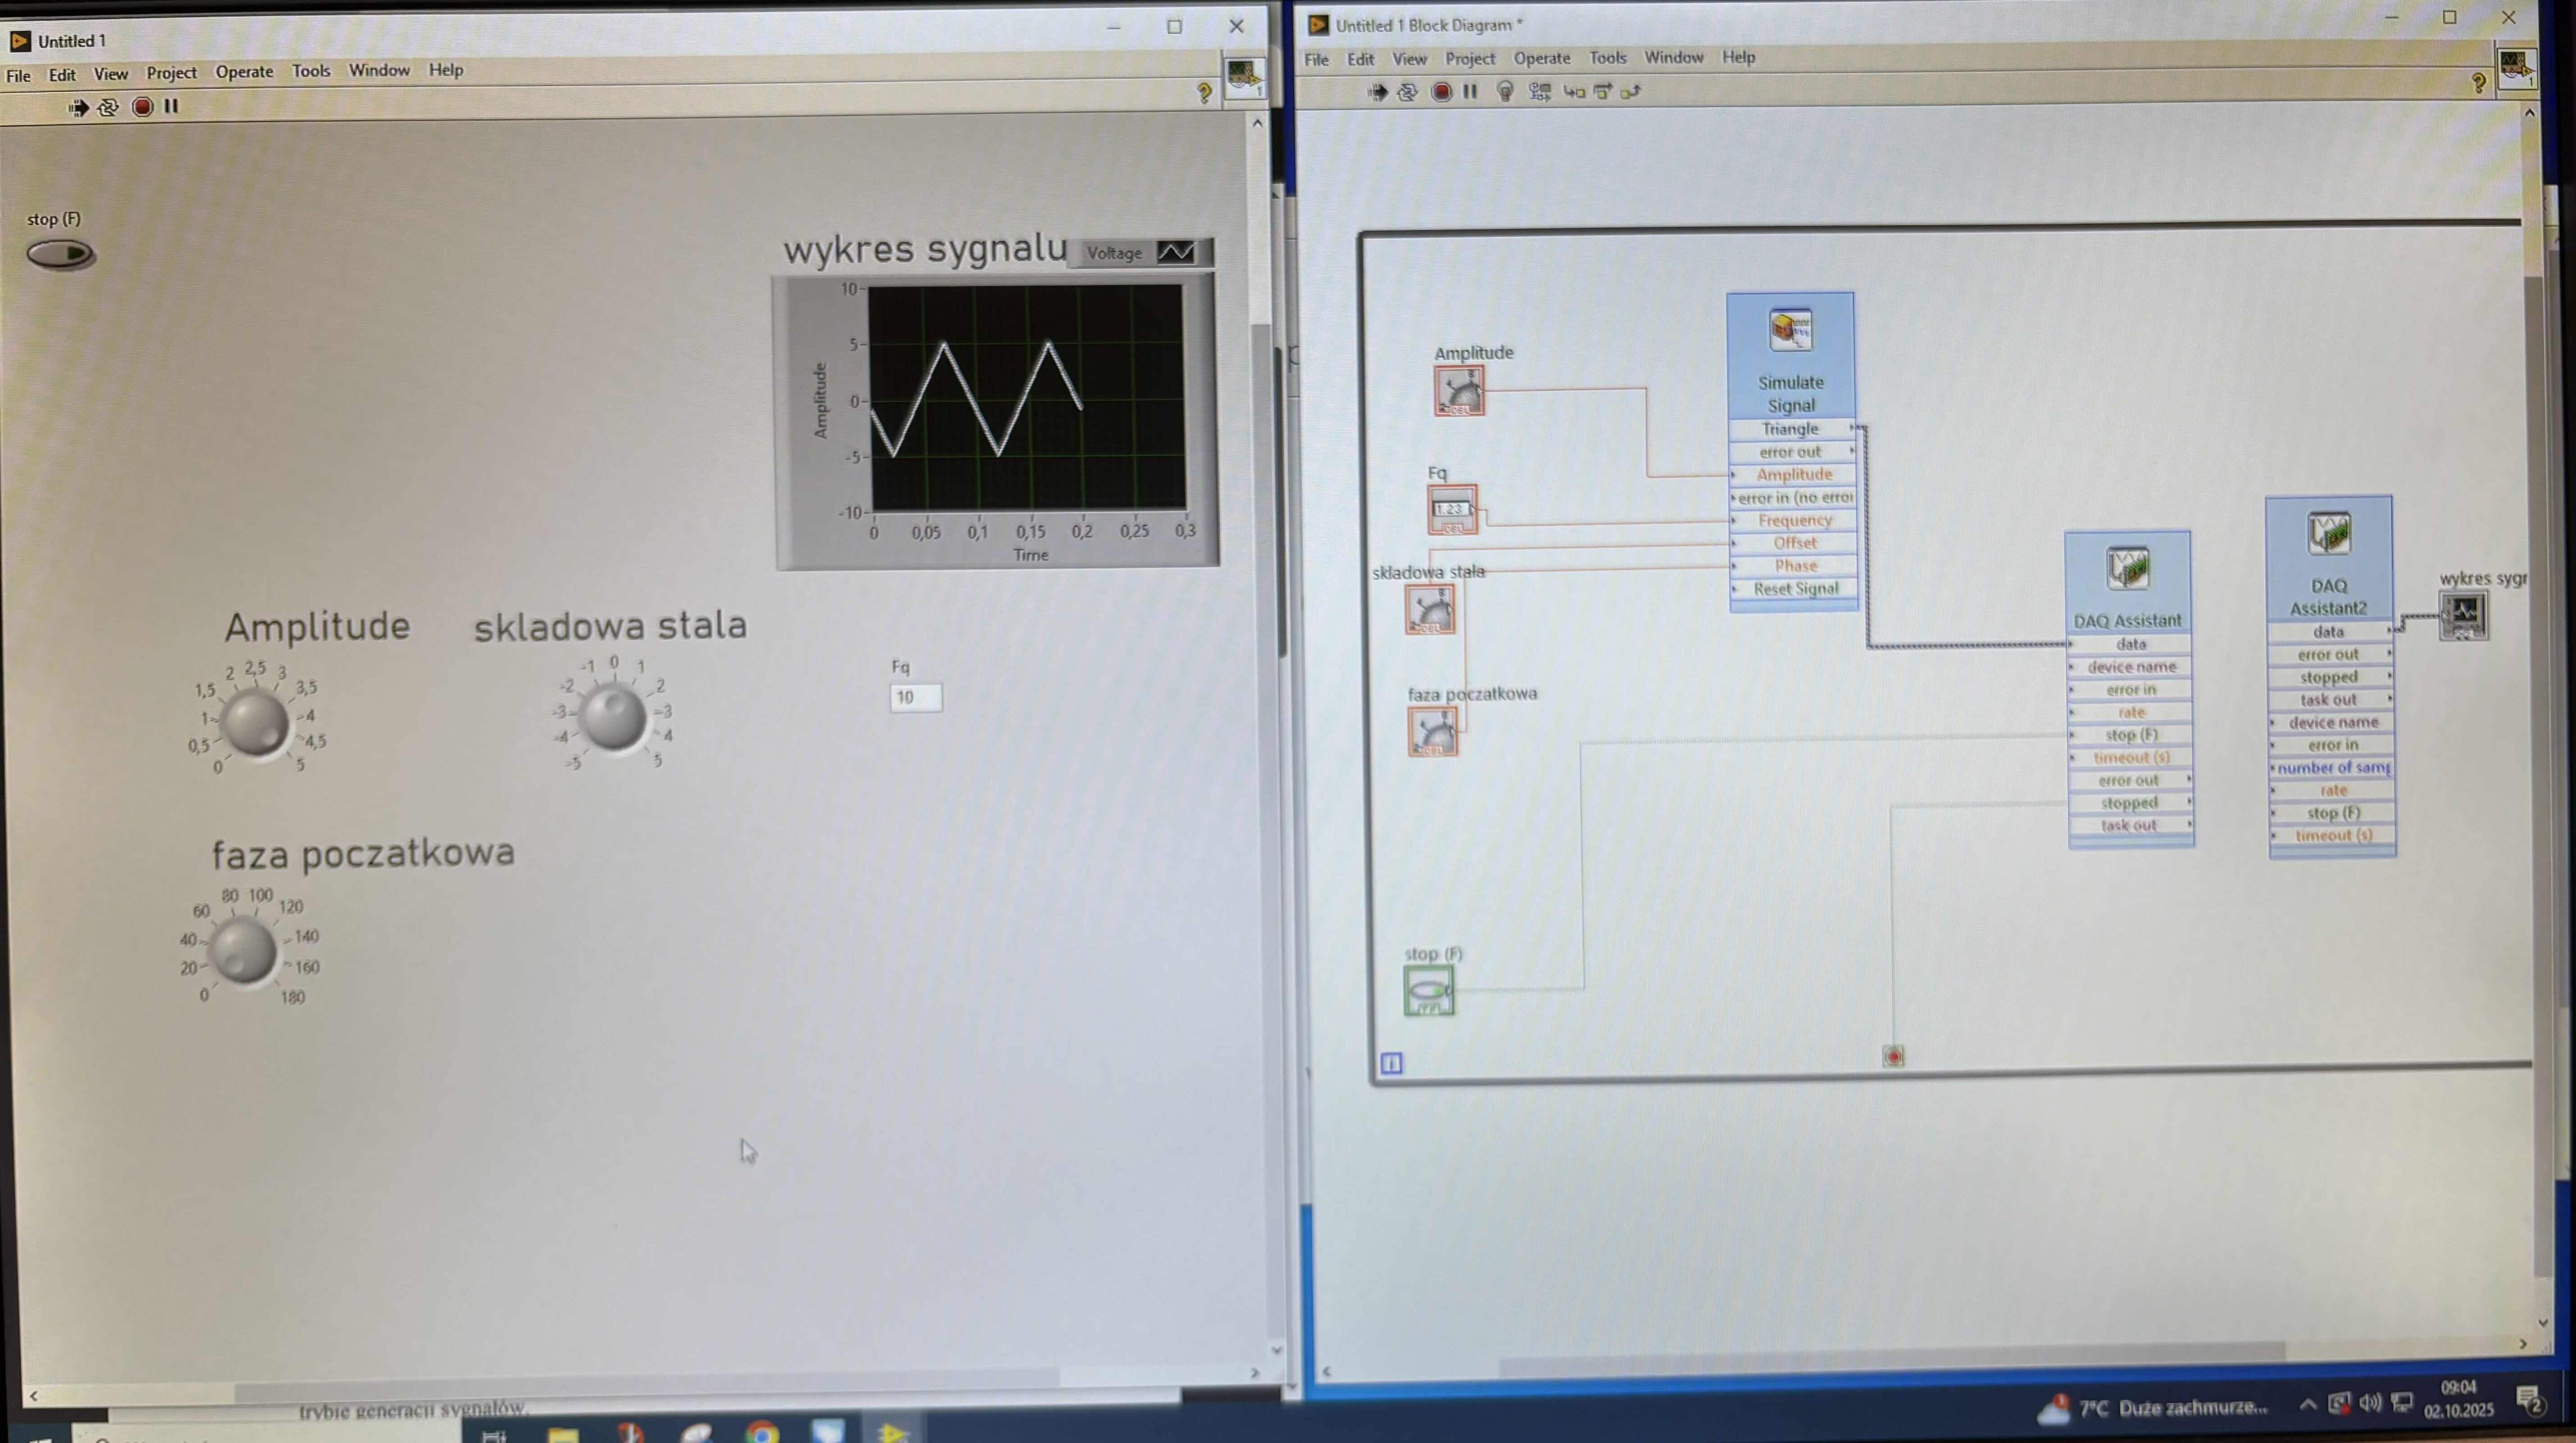
\includegraphics[width=0.5\linewidth]{img/obraz1.png}
    \caption{Gotowy układ do generacji układów w LabVIEW}
    \label{fig:placeholder}
\end{figure}

\begin{figure}[H]
  \centering
  \begin{subfigure}{.48\textwidth}
    \centering
    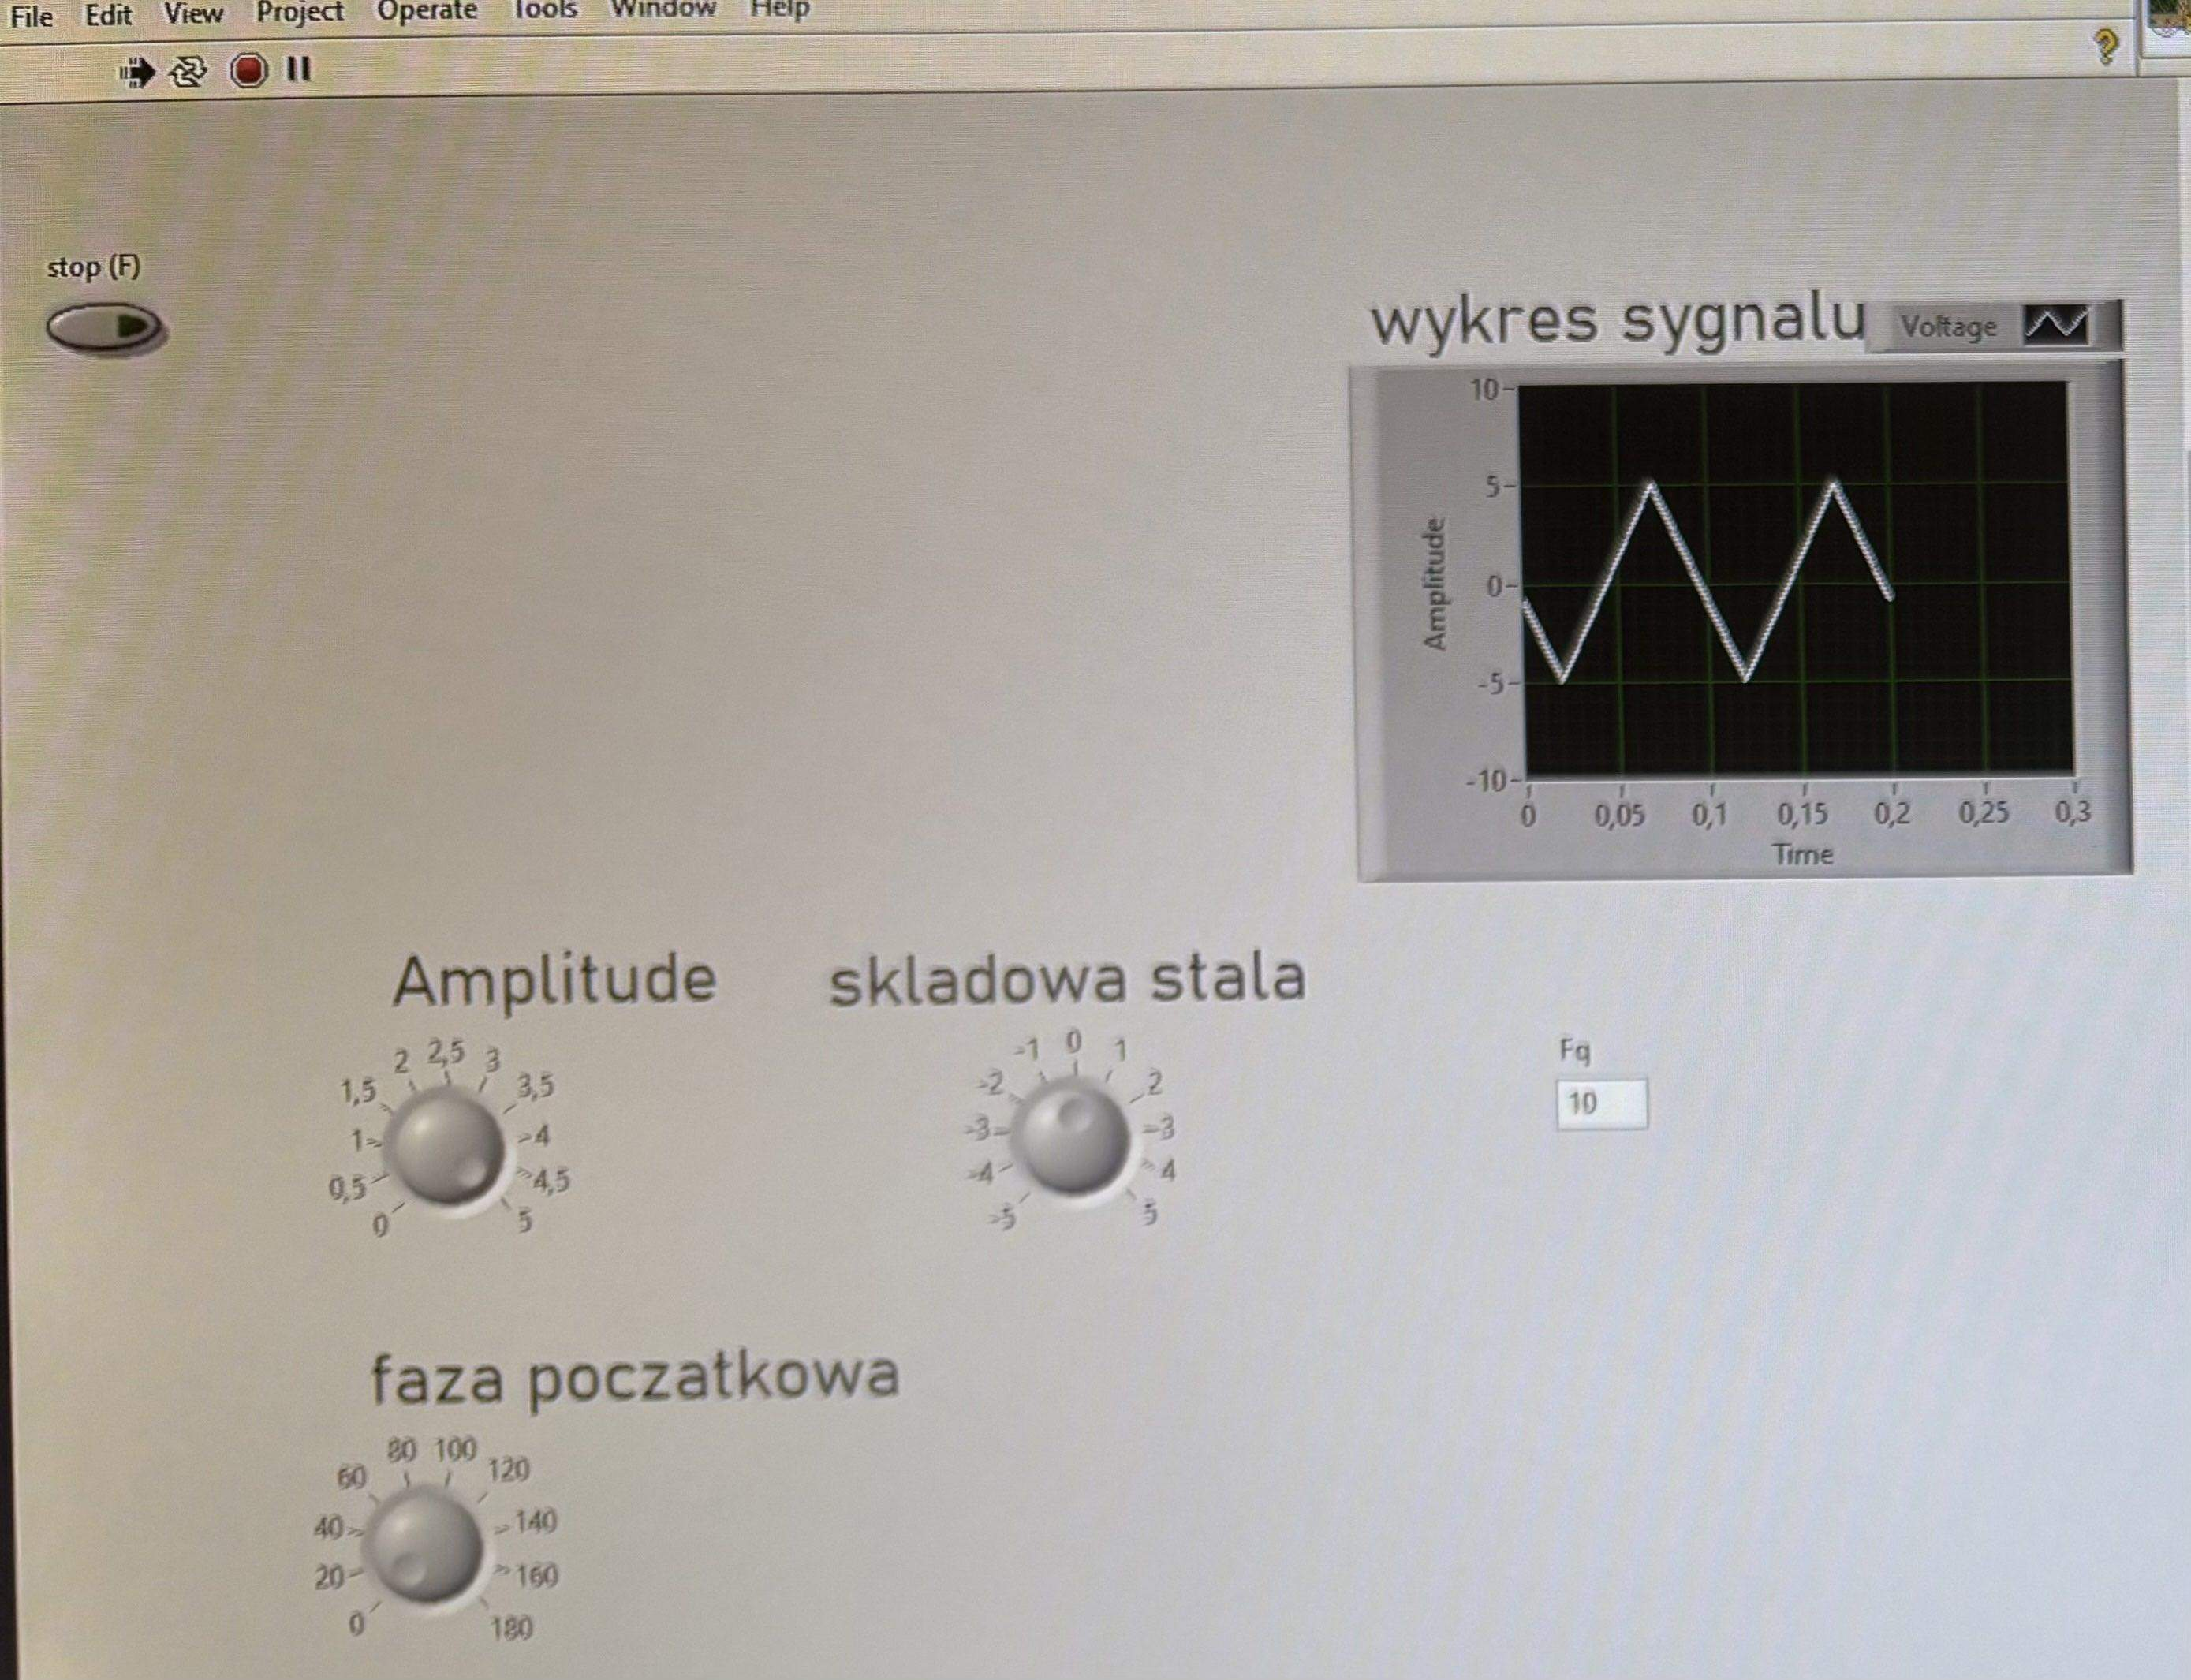
\includegraphics[width=\linewidth]{img/obraz2.png}
    \caption{Opis 1}
    \label{fig:sub1}
  \end{subfigure}\hfill
  \begin{subfigure}{.48\textwidth}
    \centering
    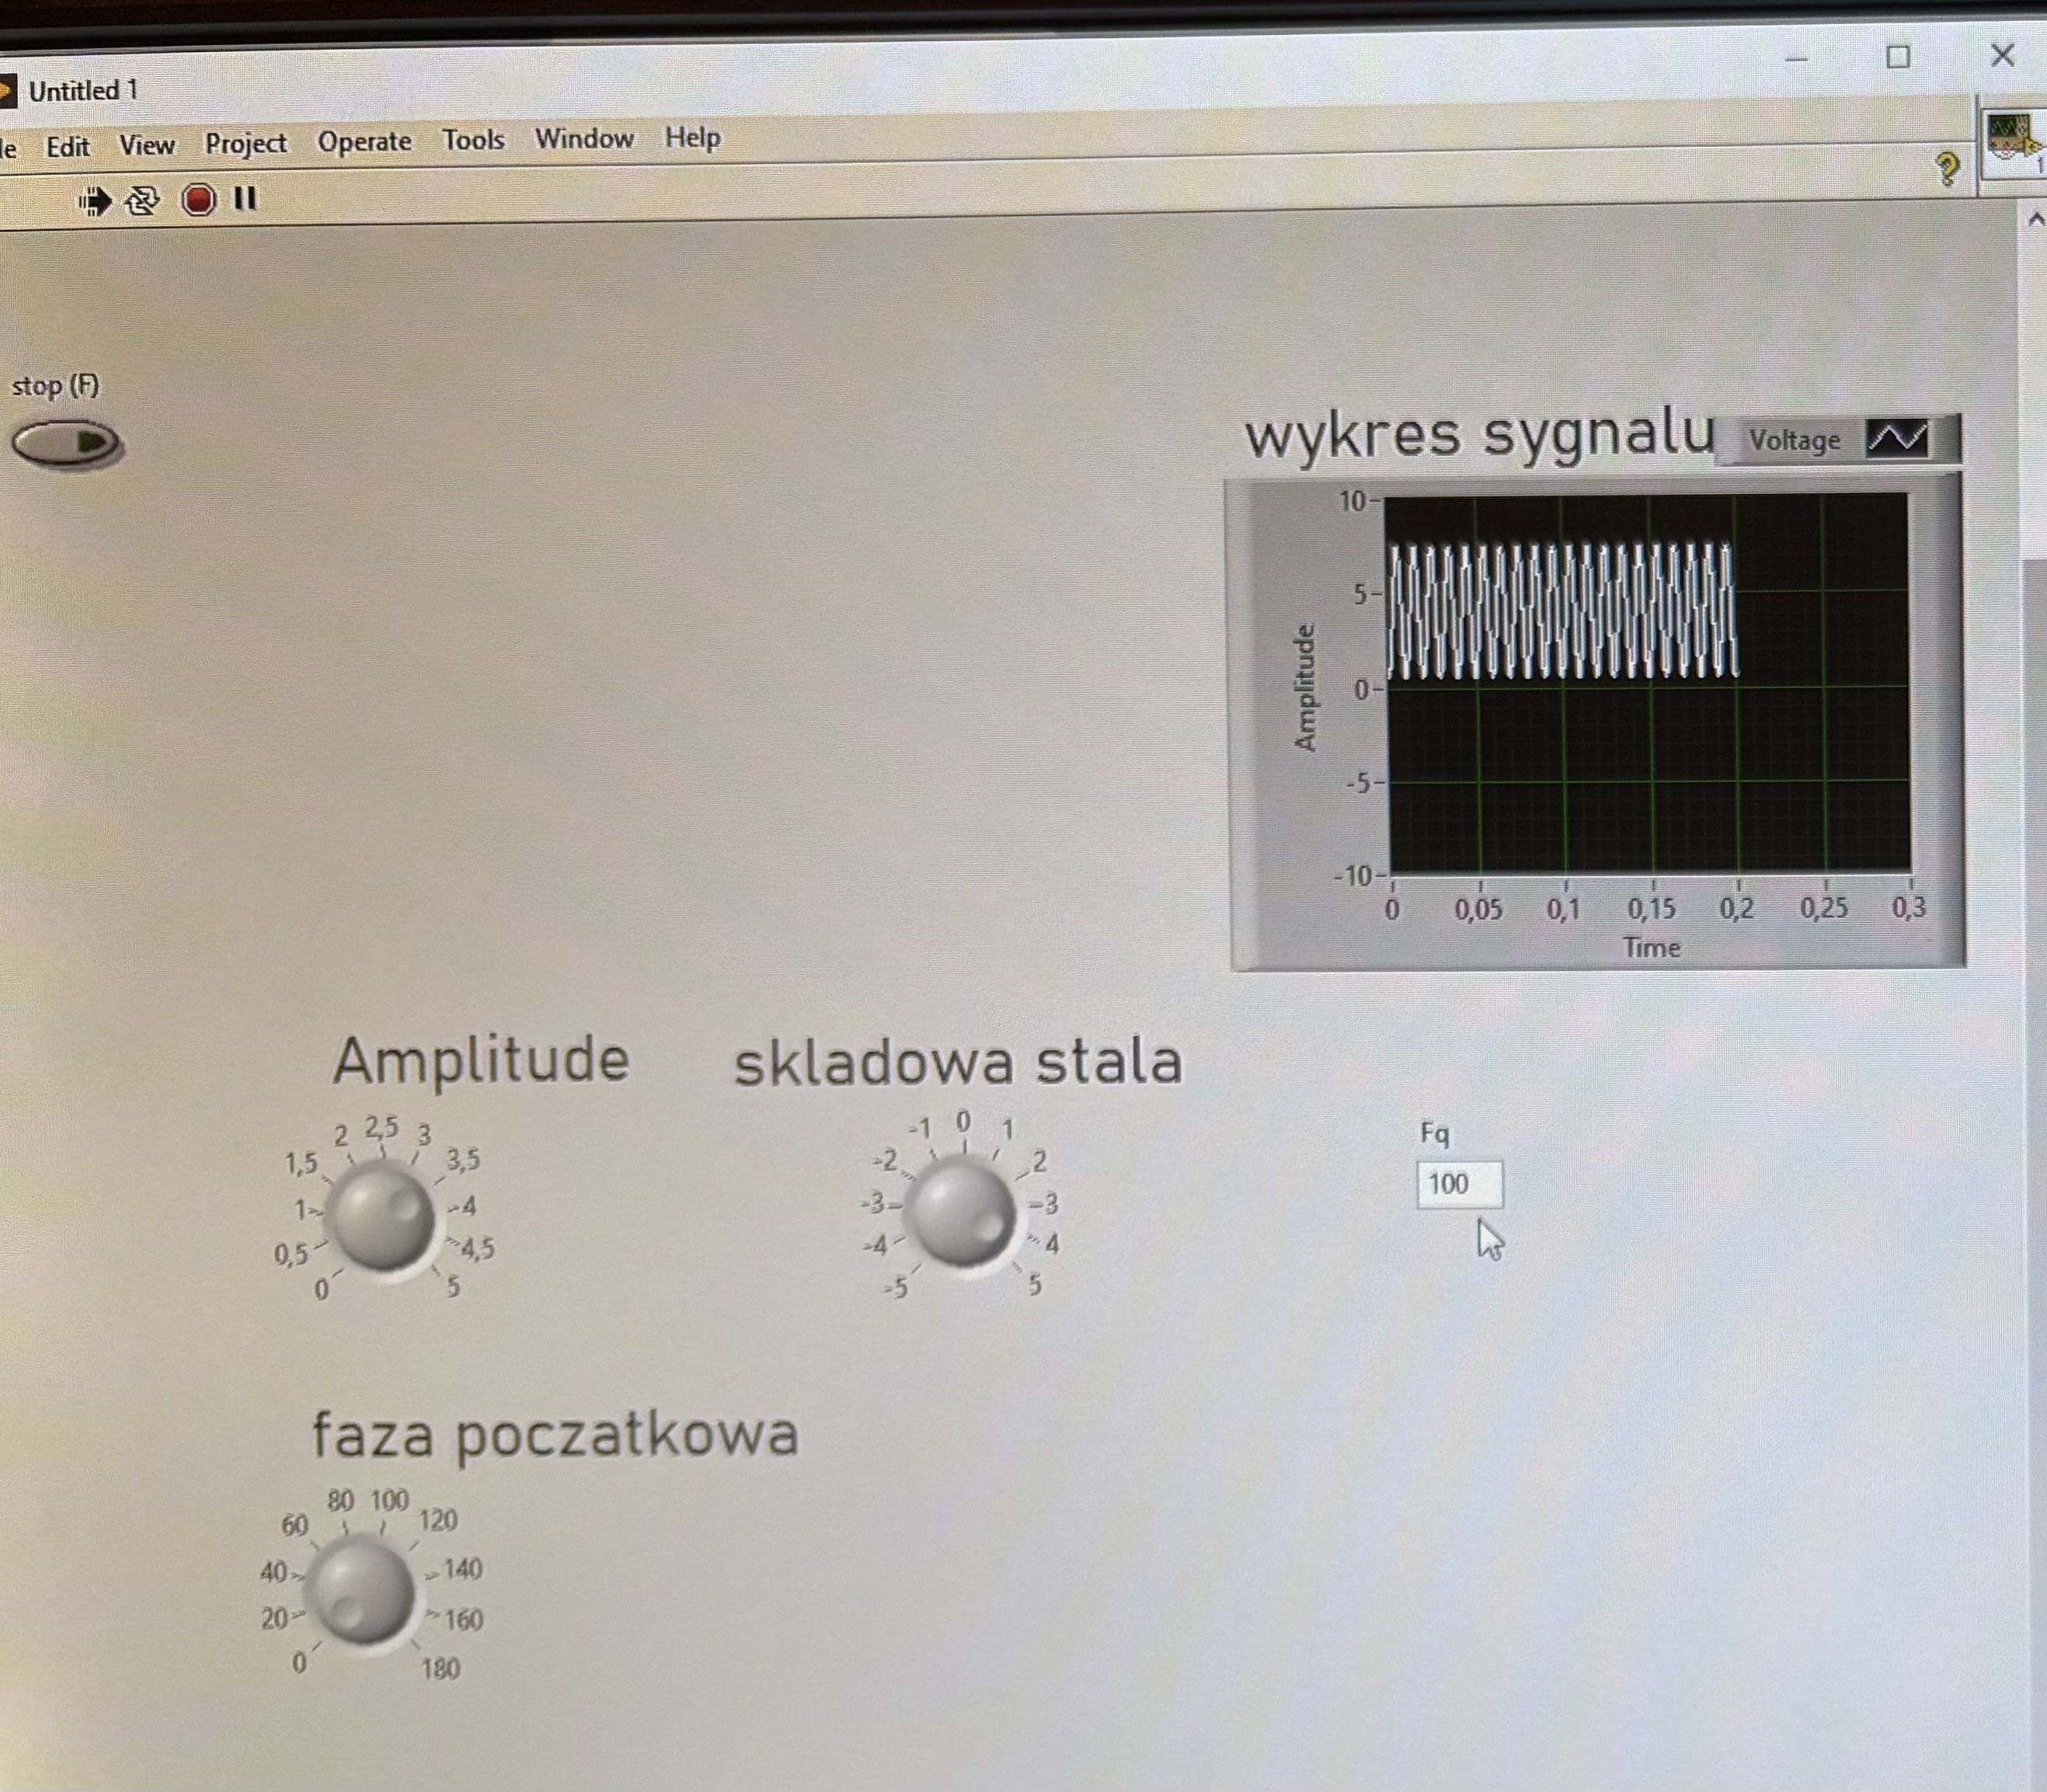
\includegraphics[width=\linewidth]{img/obraz3.png}
    \caption{Opis 2}
    \label{fig:sub2}
  \end{subfigure}

  \caption{Przebiegi sygnałów wraz z nastawami}
  \label{fig:przebiegi}
\end{figure}


\subsection{Rejestracja sygnałów}
Zmodyfikowaliśmy połączenie na płycie tak ze pomiędzy wyjściem i wejściem nieodwracającym znajduje się kondensator 

\begin{figure}[H]
    \centering
    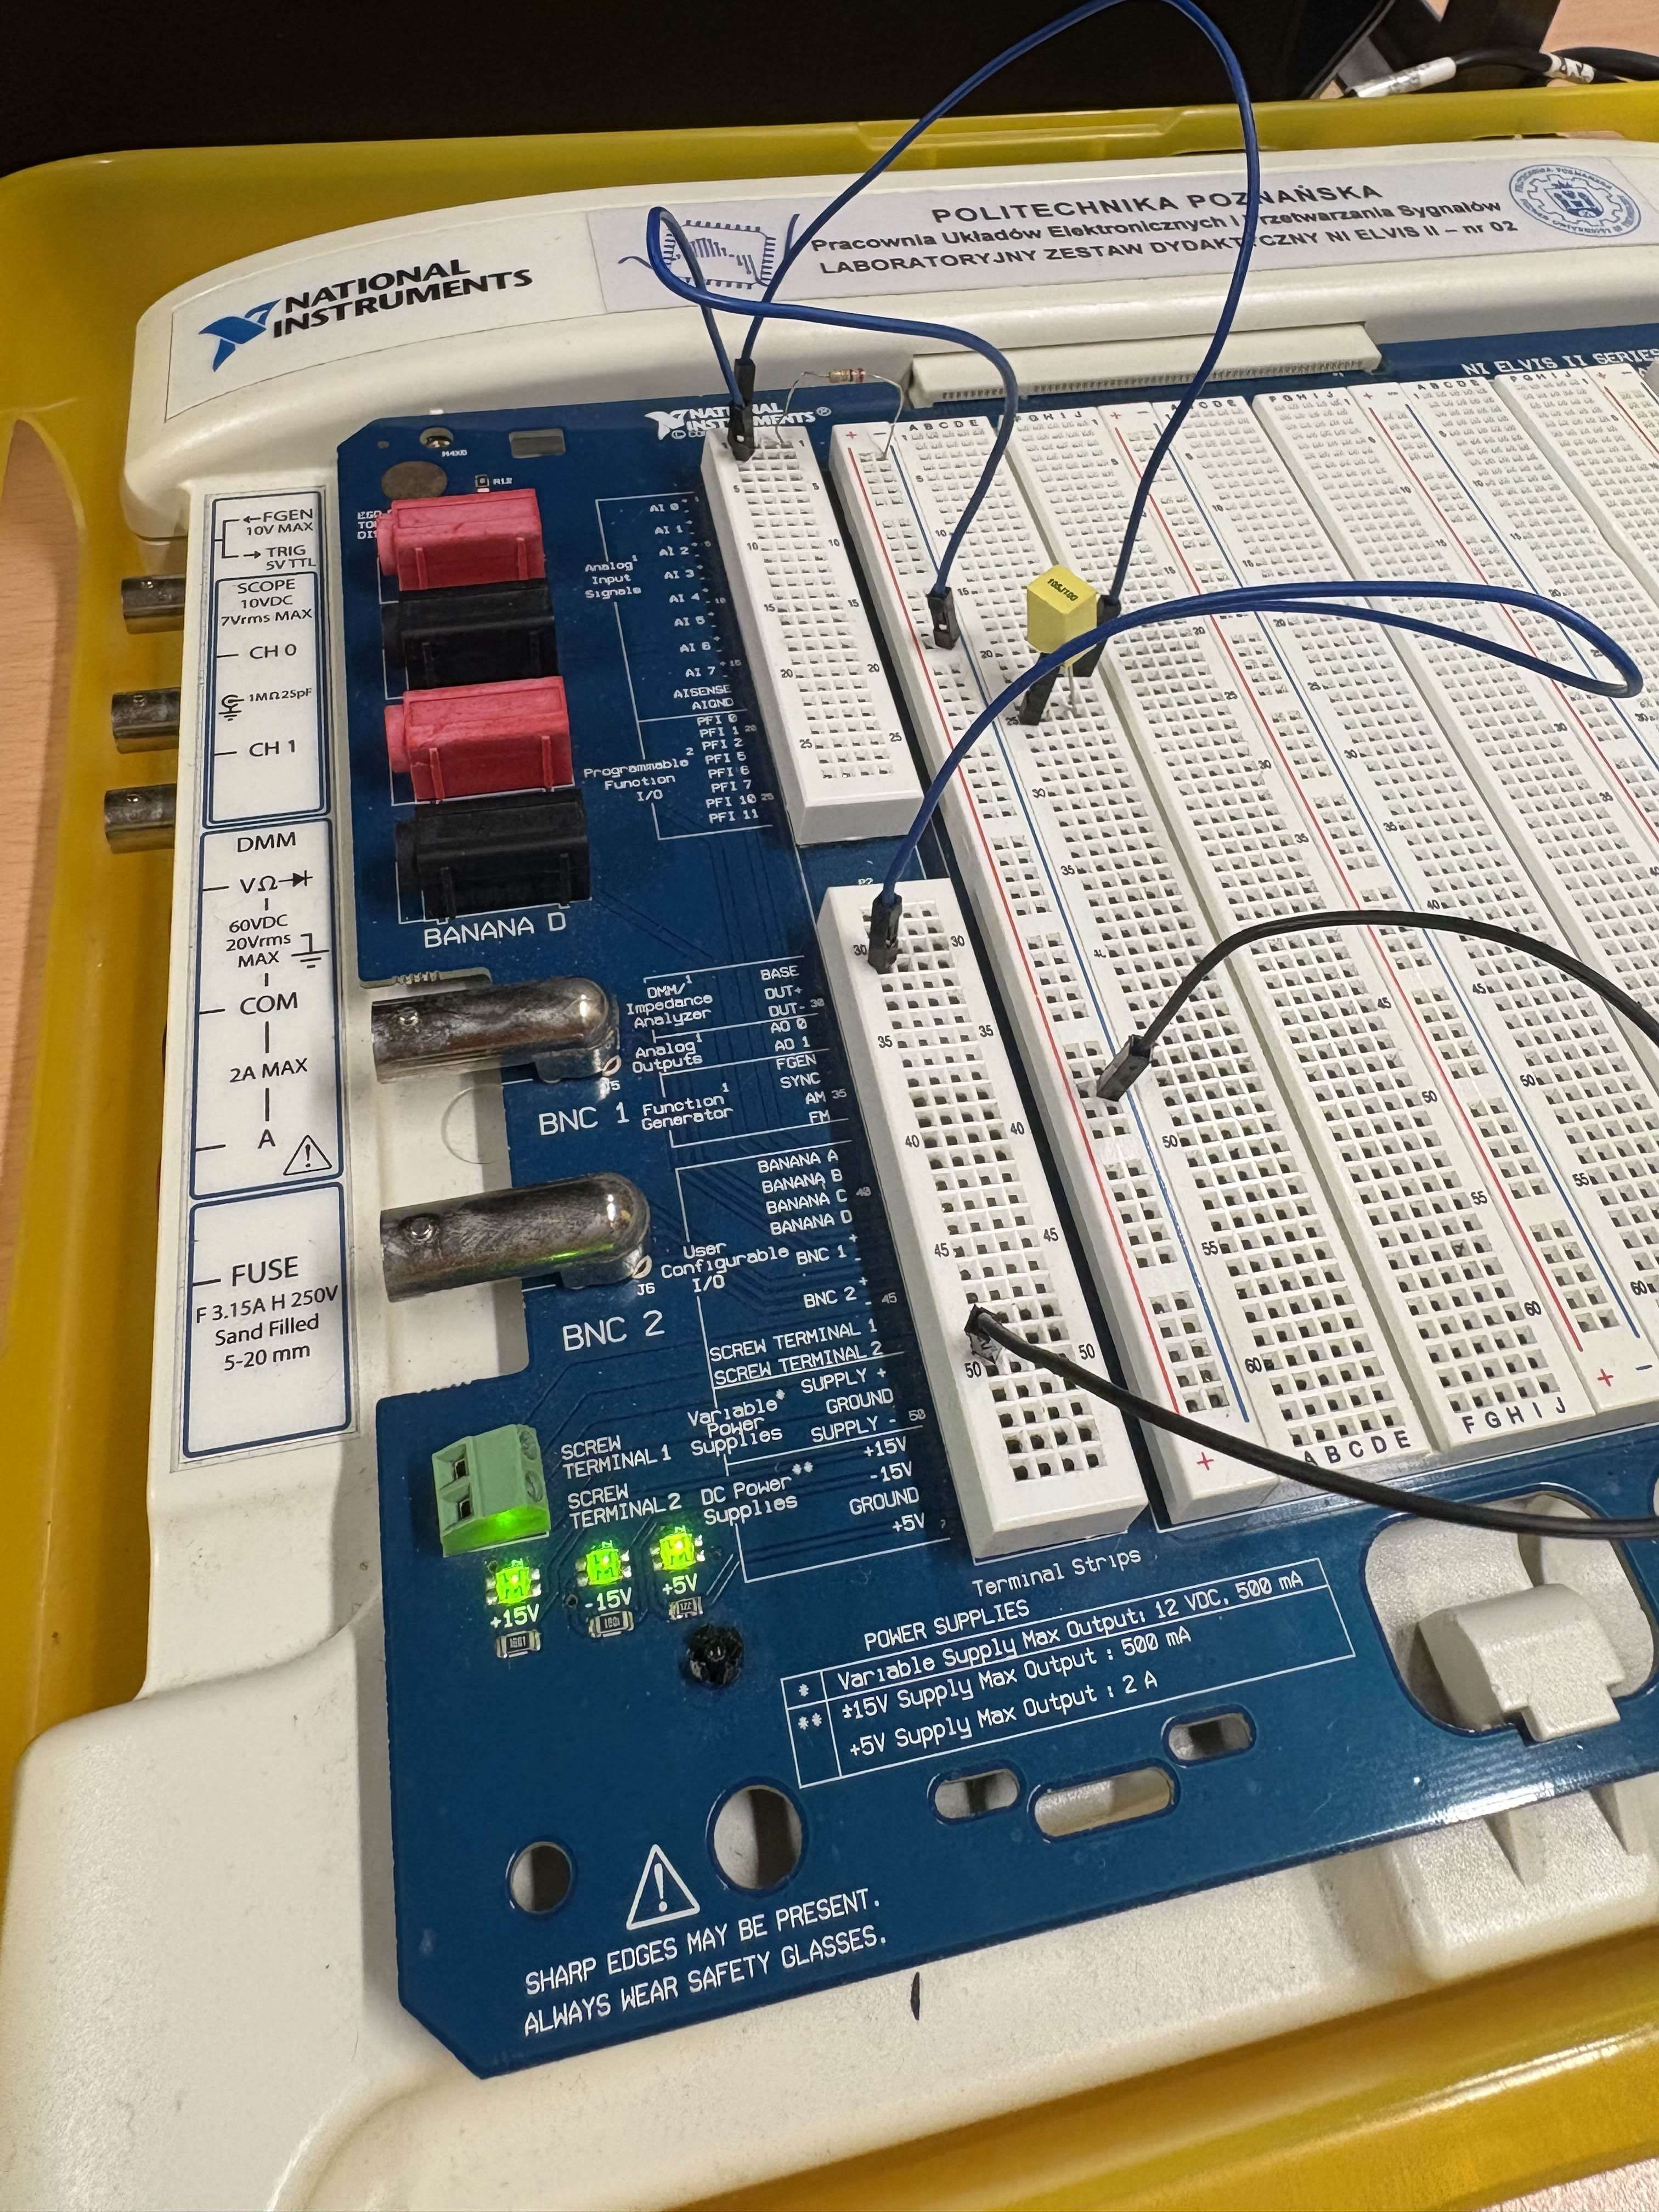
\includegraphics[width=0.5\linewidth]{img/obraz5.png}
    \caption{Enter Caption}
    \label{fig:placeholder}
\end{figure}



\end{document}

